\documentclass{beamer}

\definecolor{theme}{HTML}{2471A3}
\definecolor{accent}{HTML}{6272B5}
\definecolor{offblack}{HTML}{2E4053}
\definecolor{pyred}{HTML}{F24532}
\definecolor{pyblue}{HTML}{2E7EBC}
\definecolor{pyorange}{HTML}{FEA862}
\setbeamercolor{normal text}{fg=offblack}

\usecolortheme[named=theme]{structure}
\usecolortheme{rose}
\usecolortheme{dolphin}

% modified version of default frametitle with horizontal separation line
\makeatletter
\setbeamertemplate{frametitle}{
  \ifbeamercolorempty[bg]{frametitle}{}{\nointerlineskip}%
  \@tempdima=\textwidth%
  \advance\@tempdima by\beamer@leftmargin%
  \advance\@tempdima by\beamer@rightmargin%
  \begin{beamercolorbox}[sep=0.3cm,left,wd=\the\@tempdima]{frametitle}
    \usebeamerfont{frametitle}%
    \vbox{}\vskip-2ex%
    \if@tempswa\else\csname beamer@fteleft\endcsname\fi%
    \strut\insertframetitle\strut\par%
    {%
      \ifx\insertframesubtitle\@empty%
      \else%
      {\usebeamerfont{framesubtitle}\usebeamercolor[fg]{framesubtitle}\insertframesubtitle\strut\par}%
      \fi
    }%
    \vskip.45ex%
    \hrule %height .6pt%
    \vskip-1.45ex%
    \if@tempswa\else\vskip-.3cm\fi%
  \end{beamercolorbox}%
}
\makeatother

% clean up footer
\beamertemplatenavigationsymbolsempty
\defbeamertemplate{footline}{custom footline}{
  \usebeamercolor[fg]{page number in head/foot}
  \usebeamerfont{page number in head/foot}
  \quad
  \insertshortauthor\enskip(\insertshortinstitute)
  \hfill
  \insertshorttitle
  \hfill
  \insertframenumber\,/\,\inserttotalframenumber\kern1em\vskip2pt
}
\setbeamertemplate{footline}[custom footline]

\useinnertheme{default}

\setbeamertemplate{itemize items}[circle]
\setbeamercolor{itemize item}{fg=theme!60!white}
\setbeamercolor{itemize subitem}{fg=theme!60!white}

\usepackage{graphicx}
\usepackage[export]{adjustbox}
\usepackage{appendixnumberbeamer}
\graphicspath{{fig/}}

\usepackage[absolute]{textpos}
\usepackage{tcolorbox}

\usepackage{fontawesome}

\usepackage{tikz}
\usepackage{tikzscale}
\usetikzlibrary{calc}
\usetikzlibrary{positioning}
\usetikzlibrary{overlay-beamer-styles}
\usetikzlibrary{arrows}

\usepackage{amsmath}
\usepackage{setspace}

\usepackage[T1]{fontenc}
%% main font
\usepackage[default]{lato}
%% improves consistency of Greek letters in math mode
%\usepackage{newtxsf}

% alternate font
\usepackage[nosfdefault]{raleway}
% set as the default rm font [even though it really isn't roman]
\renewcommand*\rmdefault{Raleway-TLF}
% and use as the frame title font
\setbeamerfont{frametitle}{family=\rm}

% macros
\newcommand{\trento}{T\raisebox{-0.3ex}{R}ENTo}

\newcommand{\fullwidth}[1]{
  \begin{columns}
    \column{\paperwidth}
    #1
  \end{columns}
}

% tikz grid overlay
\newcommand{\grid}{
  \begin{tikzpicture}[remember picture, overlay]
    \draw[step=1cm, gray, very thin] (current page.south west) grid (current page.north east);
  \end{tikzpicture}
}

% place lead nucleus at tikz coordinate
\newcommand{\lead}[1]{
  \node (position) at (8.8 cm, -5 cm) {\includegraphics[scale=0.27]{#1}};
}

% place lead nucleus at tikz coordinate
\newcommand{\pic}[3]{
  \node (position) at #2 {\includegraphics[scale=#3]{#1}};
}

\newcommand{\tran}{^\intercal}
\newcommand{\T}{\tilde{T}}

\title[Bayesian parameter estimation for HIC]{Bayesian parameter estimation for heavy-ion collisions: inferring properties of the quark-gluon plasma}
\author[J.\ S.\ Moreland]{J.\ Scott Moreland}
\institute[Duke U.]{Duke Univerity}
\date{\today}

\begin{document}

\section{Title}


\begin{frame}[t,plain,noframenumbering]
  \centering \vspace{.3\textheight}
  {\color{theme}\large\rm\inserttitle} \\[.04\textheight]
  {\small \insertauthor---Duke U.} \\[1ex]
  {\small XLVII International Symposium on Multiparticle Dynamics\\September 14, 2017}
\end{frame}


\begin{frame}{Lattice predicts existence of a quark-gluon plasma}
  Lattice QCD calculations find a pseudo-critical phase transition temperature $T \approx 155$~MeV, where hadrons melt to form a deconfined soup of quarks and gluons dubbed a quark-gluon plasma (QGP)\\[2ex]
  \begin{columns}
    \begin{column}{0.47\textwidth}
        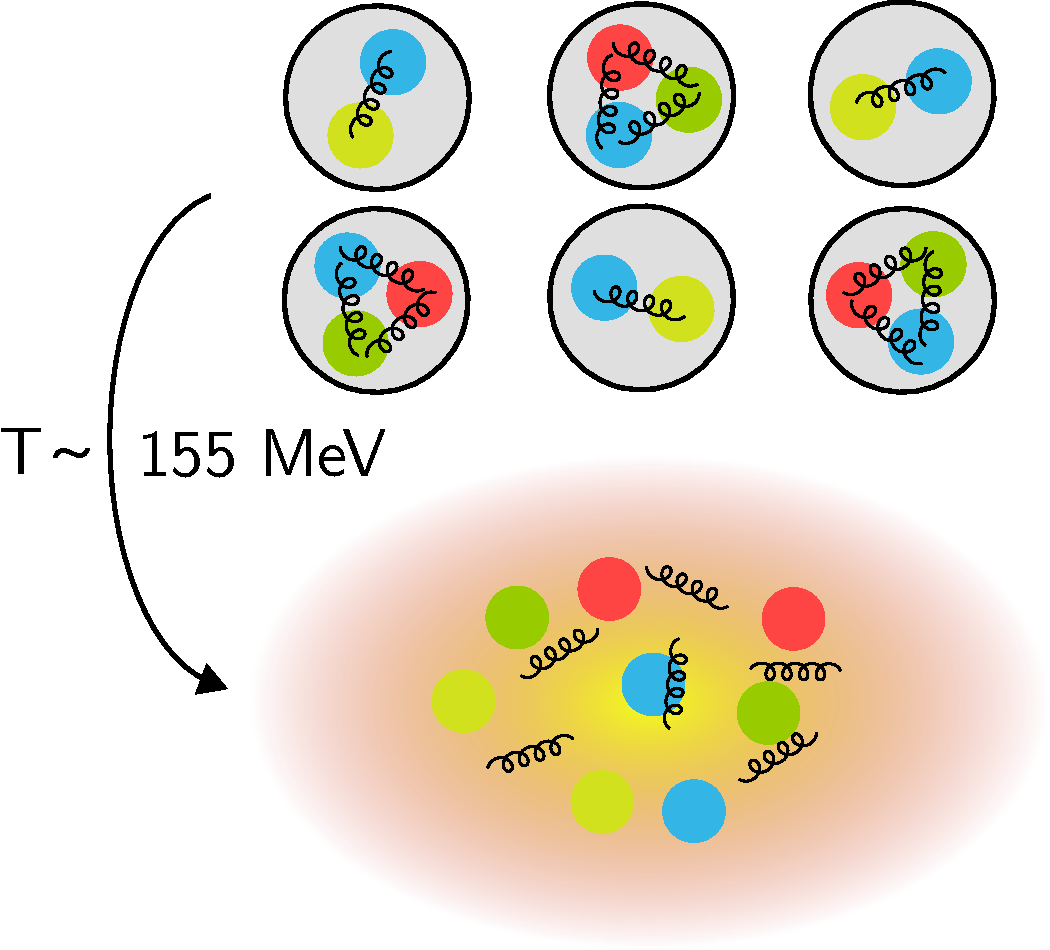
\includegraphics[width=\columnwidth]{confined_deconfined}
    \end{column}
    \begin{column}{0.4\textwidth}
        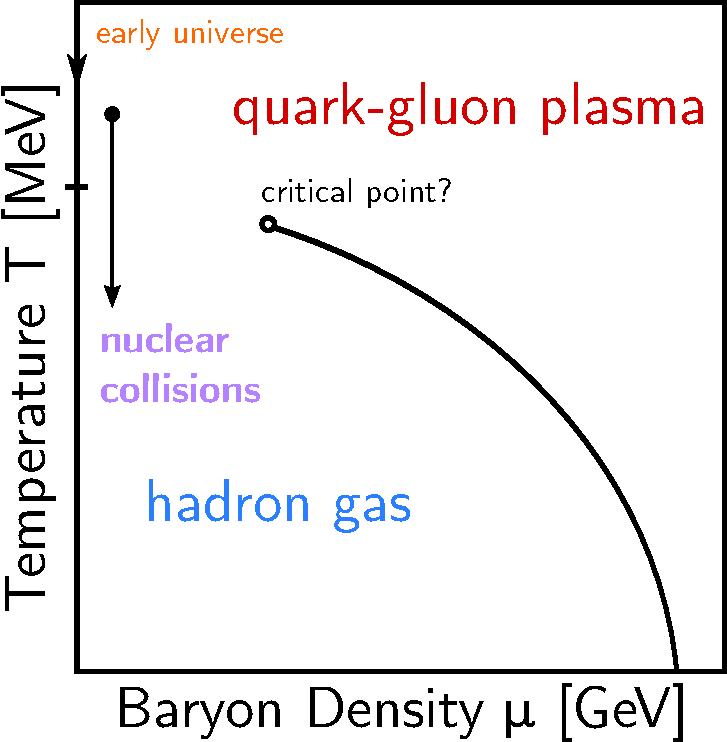
\includegraphics[width=\columnwidth]{phasediagram}
    \end{column}
  \end{columns}
\end{frame}

\begin{frame}{What are the quark-gluon plasma bulk properties?}
    \begin{center}
        \begin{tikzpicture}
            \node[anchor=center, yshift=0.75cm] (qgp) at (current page.center) {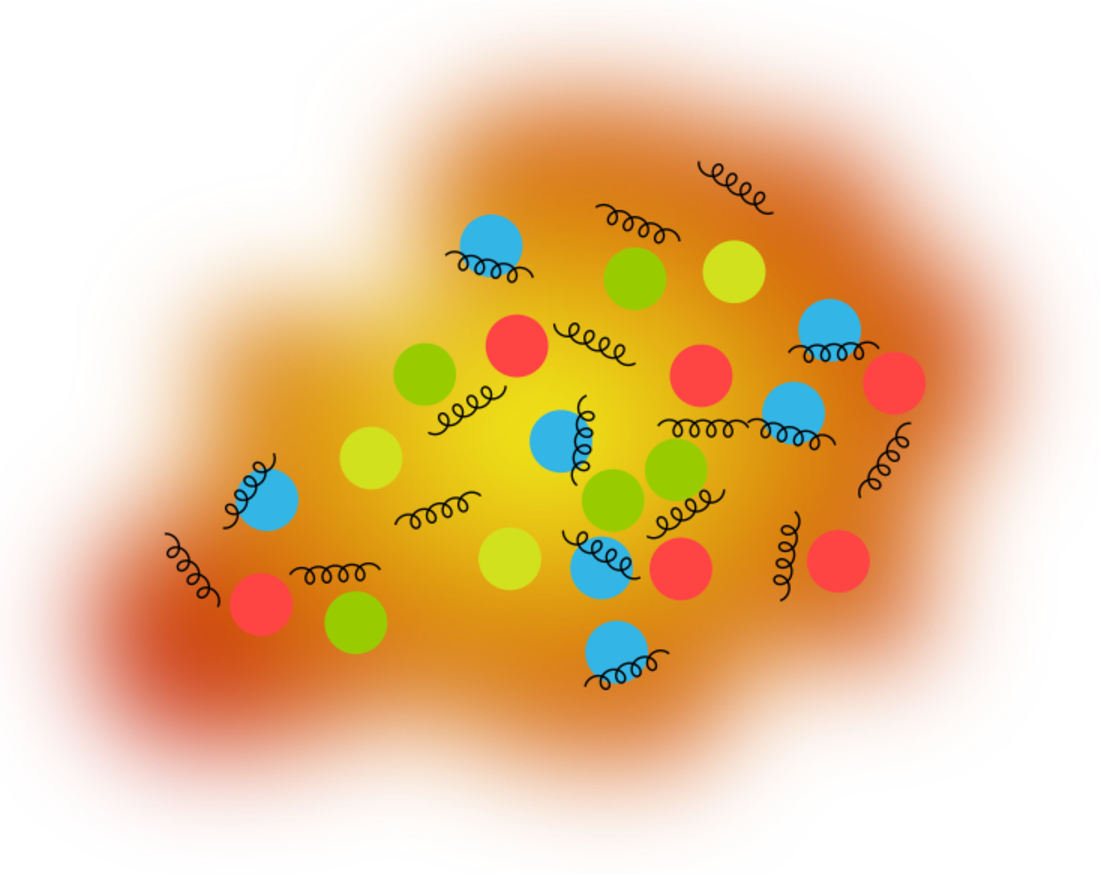
\includegraphics[width=0.35\textwidth]{qgp}};
            \node[text width=4cm, xshift=3.5cm, yshift=3.5cm] (t1) at (current page.center) {How and under what\\ conditions is it formed\\ in a nuclear collision?};
            \node[text width=4.75cm, xshift=3.5cm, yshift=-1.5cm] (t2) at (current page.center) {How does it recombine\\ to form colorless hadrons?};
            \node[text width=4cm, xshift=-3.5cm, yshift=3cm] (t3) at (current page.center) {Equation of state?\\ Relations between\\ thermal quantities,\\ e.g.\ $P=P(\epsilon)$};
            \node[text width=4cm, xshift=-3.5cm, yshift=-2cm] (t4) at (current page.center) {Transport properties?\\ shear/bulk viscosity,\\ probe energy loss, etc};
            \path[->, >=stealth, theme] ([xshift=-.1cm]t1.west) edge [out=-180, in=90] (qgp.north);
            \path[->, >=stealth, theme] ([yshift=.1cm]t2.north) edge [out=90, in=-30] (qgp.east);
            \path[->, >=stealth, theme] ([xshift=-.8cm]t3.south) edge [out=-90, in=180] (qgp.west);
            \path[->, >=stealth, theme] (t4.east) edge [out=0, in=-90] (qgp.south);
        \end{tikzpicture}
    \end{center}
\end{frame}


\begin{frame}{Formulating an inverse problem}
  \begin{center}
    \only<1>{{\scshape Model-to-data comparison (in an ideal world)} \\[5ex]}
    \only<2>{{\scshape Realistic model-to-data comparison} \\[5ex]}
  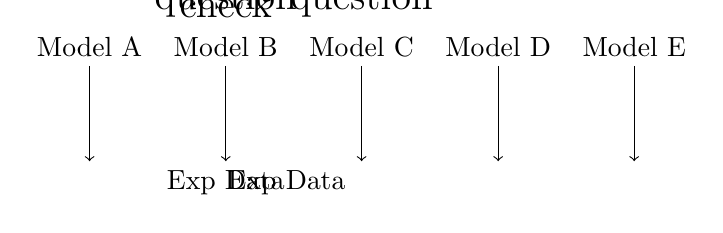
\begin{tikzpicture} 
    \node<1->[align=left] (a1) at (current page.center){Model A};
    \node<1->[right = 1ex of a1] (b1) {Model B};
    \node<1->[right = 1ex of b1] (c1) {Model C};
    \node<1->[right = 1ex of c1] (d1) {Model D};
    \node<1->[right = 1ex of d1] (e1) {Model E};

    \node<1>[above = 0ex of b1, overlay] {\Large \faicon{check}};
    \node<2>[above = 0ex of b1, overlay] {\Large \faicon{question}};
    \node<2>[above = 0ex of c1, overlay] {\Large \faicon{question}};

    \node[below = 8ex of a1] (a2) {};
    \node[below = 8ex of b1] (b2) {};
    \node[below = 8ex of c1] (c2) {};
    \node[below = 8ex of d1] (d2) {};
    \node[below = 8ex of e1] (e2) {};

    \node<1>[below = 8ex of b1] (exp) {Exp Data};
    \node<2->[below = 8ex of b1, xshift = 5.1ex] (exp) {Exp Data};

    \draw<1->[->] (a1) edge (a2);
    \draw<1->[->] (b1) edge (b2);
    \draw<1->[->] (c1) edge (c2);
    \draw<1->[->] (d1) edge (d2);
    \draw<1->[->] (e1) edge (e2);
  \end{tikzpicture}\\
  \end{center}
\end{frame}


\begin{frame}[plain, noframenumbering]
  \begin{center}
    \scshape \large I) Bayesian parameter estimation
  \end{center}
\end{frame}


\begin{frame}{Formulating an inverse problem}
  \begin{center}
    \only<1>{{\scshape Parametrize Theory landscape} \\[5ex]}
    \only<2-4>{{\scshape Bayesian parameter estimation} \\[5ex]}
  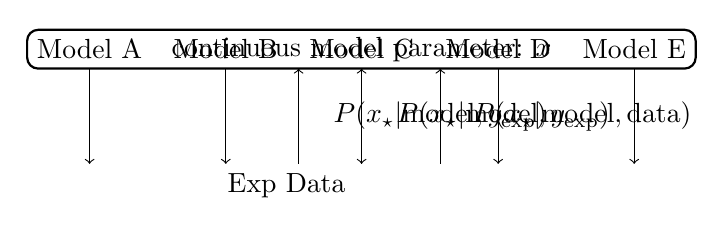
\begin{tikzpicture} 
    \node<1>[align=left] (a1) at (current page.center){Model A};
    \node<1>[right = 1ex of a1] (b1) {Model B};
    \node<1>[right = 1ex of b1] (c1) {Model C};
    \node<1>[right = 1ex of c1] (d1) {Model D};
    \node<1>[right = 1ex of d1] (e1) {Model E};
    \node<2-4>[align=center] at (c1) {continuous model parameter: $x$};

    \node[below = 8ex of a1] (a2) {};
    \node[below = 8ex of b1] (b2) {};
    \node[below = 8ex of c1] (c2) {};
    \node[below = 8ex of d1] (d2) {};
    \node[below = 8ex of e1] (e2) {};

    \node<1-4>[below = 8ex of b1, xshift = 5.1ex] (exp) {Exp Data};

    \draw<1>[->] (a1) edge (a2);
    \draw<1>[->] (b1) edge (b2);
    \draw<1>[->] (c1) edge (c2);
    \draw<1>[->] (d1) edge (d2);
    \draw<1>[->] (e1) edge (e2);

    \draw<1-4>[thick, rounded corners, overlay] (a1.south west) rectangle (e1.north east);

    \draw<2>[->, transform canvas={xshift=1cm}] (c2) edge (c1);
    \node<2>[below=2ex of c1, transform canvas={xshift=2.8cm}]
    {$P(x_\star| \text{model}, \text{data})$};

    \draw<3>[->, transform canvas={xshift=0cm}] (c2) edge (c1);
    \node<3>[below=2ex of c1, transform canvas={xshift=1.8cm}]
    {$P(x_\star| \text{model}, y_\text{exp})$};

    \draw<4>[->, transform canvas={xshift=-0.8cm}] (c2) edge (c1);
    \node<4>[below=2ex of c1, transform canvas={xshift=1cm}]
    {$P(x_\star| \text{model}, y_\text{exp})$};

    \node<2-4>[below=4ex of c2, overlay, align=center]
    {{\scshape Bayes' Theorem:}\\$\underbrace{P(x_\star| \text{model},\text{data})}_\text{posterior} \propto \underbrace{P(\text{model},\text{data}|x_\star)}_\text{likelihood}\underbrace{P(x_\star)}_\text{prior}$};
  \end{tikzpicture}\\
    \only<5>{
      {\scshape Yields posterior distribution on $x_\star$}\\[2ex]
      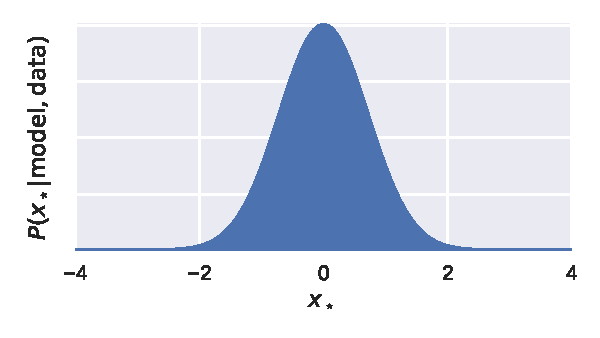
\includegraphics[scale=.8]{bayes}\\
      \emph{Includes uncertainty in ``best-fit value''}
    }
  \end{center}
\end{frame}


\begin{frame}{Multiple observables}
  \begin{center}
    {\large posterior = likelihood $\times$ prior}\\[2ex]
    More than one observable $f: x \mapsto (y_1, ..., y_n)$?\\
    No problem, calculate likelihood using multivariate Gaussian
  \end{center}
  \begin{block}{Log-likelihood}
    \vspace{-3ex}
    \begin{align*}
      \ln(L) &= -\frac{1}{2}(\ln(|\boldsymbol{\Sigma}|) + (\mathbf{y} - \mathbf{y}_\text{exp})^T \boldsymbol{\Sigma}^{-1} (\mathbf{y} - \mathbf{y}_\text{exp}) + k \ln(2\pi))\\
      \boldsymbol{\Sigma} &= \boldsymbol{\Sigma}_\text{model} + \boldsymbol{\Sigma}_\text{exp}^\text{stat} + \boldsymbol{\Sigma}_\text{exp}^\text{sys}
    \end{align*}
  \end{block}
\end{frame}


\begin{frame}{Multiple model parameters}
  \begin{center}
    {\large posterior = likelihood $\times$ prior}\\[2ex]
    Likelihood function $L(x) \rightarrow L(x_1, ...,x_n)$
  \end{center}
  \begin{columns}[t]
    \begin{column}{0.5\textwidth}
      \begin{block}{Curse of dimensionality}
        Typically interested in marginalized probabilities\\[1ex]
        $L(x_1,...,x_n)$ easy to calculate,\\
        hard to integrate.
      \end{block}

      \begin{block}{Solution}
        Monte Carlo integration,
        e.g.\ importance sampling
      \end{block}
    \end{column}
    \vline
    \begin{column}{0.5\textwidth}
      \begin{center}
        {\color{theme} MCMC importance sampling:}\\[1ex]
        \begin{enumerate}
          \item large number of walkers in $\{x_1,...,x_n\}$ space
          \item perturb walker positions
          \item accept new $\mathbf x$ with prob\\
            $P \sim L_\text{new} / L_\text{old}$
        \end{enumerate}
        Marginalize by histogramming over flattened dimensions
      \end{center}
    \end{column}
  \end{columns}
\end{frame}


\begin{frame}{MCMC and evaluating the likelihood}
  \begin{center}
    Number of likelihood samples needed for MCMC varies greatly
  \end{center}
  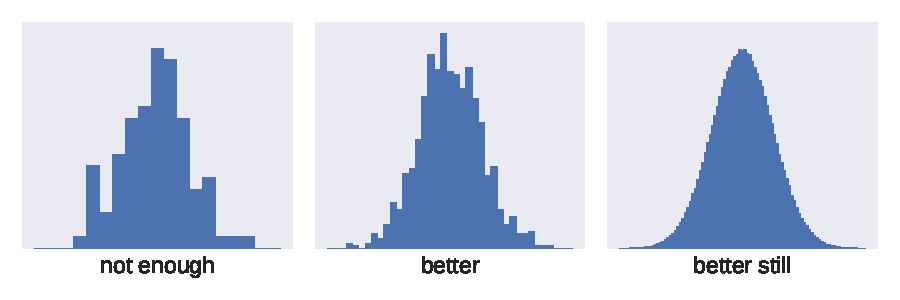
\includegraphics[width=\textwidth]{mcmc}\\
  \begin{center}
    Several of the published results in this talk use $N_\text{sample} > 10^6$\\
    If model is slow, e.g.\ 1 CPU hour per likelihood evaluation\\
    \faicon{clock-o} ...good luck
  \end{center}
\end{frame}


\begin{frame}{Training an emulator}
  \vspace{1em}
  \begin{columns}[c]
    \column{.58\textwidth}
    Gaussian process:
    \begin{itemize}
      \item Stochastic function: maps inputs to normally-distributed outputs
      \item Specified by mean and covariance functions
    \end{itemize}
    \bigskip
    As a model emulator:
    \begin{itemize}
      \item Non-parametric interpolation
      \item Predicts \emph{probability distributions}
        \begin{itemize}
          \item Narrow near training points, \\ wide in gaps
        \end{itemize}
      \item Fast surrogate to actual model
    \end{itemize}
    \column{.45\textwidth}
    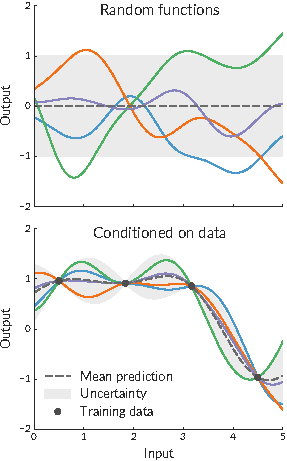
\includegraphics{gp}
  \end{columns}
\end{frame}


\begin{frame}{Workflow}
  \begin{flushleft}
    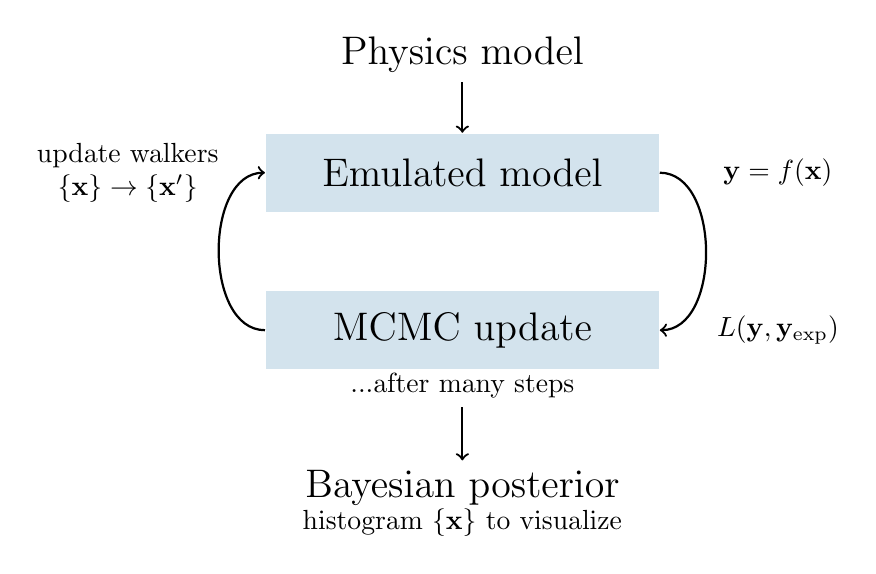
\begin{tikzpicture}
      \node[align=center] (x1) at (current page.center) {\Large Physics model};
      \node[rectangle, draw=white, fill=theme!20, align=center, yshift=-1.5cm, minimum width=5cm, minimum height=1cm] (x2) at (current page.center) {\Large Emulated model};
      \node[rectangle, draw=white, fill=theme!20, align=center, yshift=-2cm, minimum width=5cm, minimum height=1cm] (x3) at (x2.center) {\Large MCMC update};
      \node[align=center, xshift=-4.25cm, yshift=0cm] (x4) at (x2.center) {update walkers\\$\{\mathbf{x}\} \rightarrow \{\mathbf{x'}\}$};
      \node[align=center, yshift=-2cm] (x5) at (x3.center) {\Large Bayesian posterior};
      \node[align=left, xshift=1.5cm] (x6) at (x2.east) {$\mathbf{y}=f(\mathbf{x})$};
      \node[align=left, xshift=1.5cm] (x7) at (x3.east) {$L(\mathbf{y}, \mathbf{y}_\text{exp})$};
      \node[align=center, yshift=-0.7cm] (x8) at (x3.center) {...after many steps};
      \node[align=center, yshift=-.1cm] (x9) at (x5.south) {histogram $\{\mathbf{x}\}$ to visualize};
      \draw[->, thick] (x1) edge (x2);
      \draw[->, thick] (x8) edge (x5);
      \draw[->, thick] (x2.east) to [out=0, in=360] (x3.east);
      \draw[->, thick] (x3.west) to [out=180, in=-180] (x2.west);
    \end{tikzpicture}
  \end{flushleft}
\end{frame}


\begin{frame}{Bayesian parameter estimation in physics}
  \bigskip
  \begin{columns}
    \begin{column}{0.4\textwidth}
      \centering {\scshape LIGO Experiment}\\
      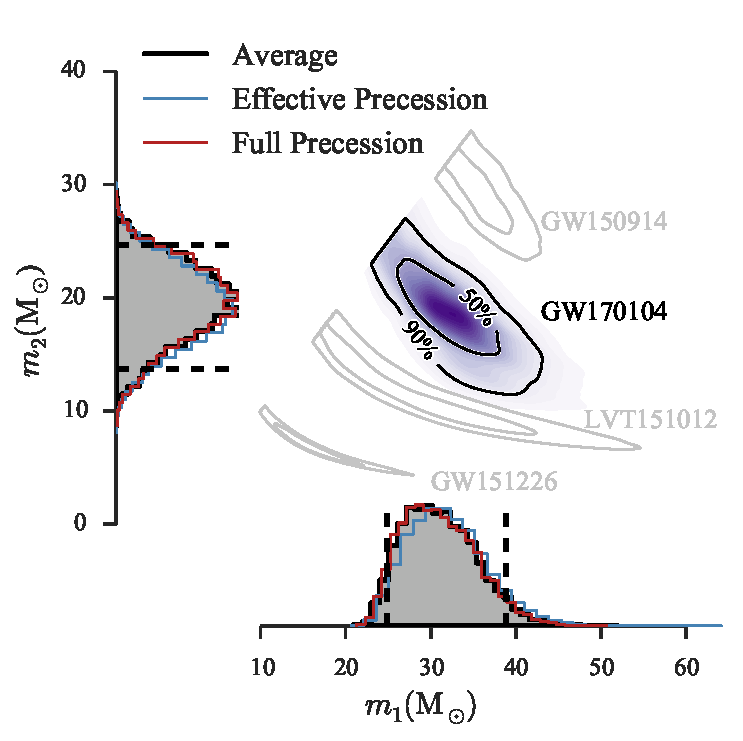
\includegraphics[width=\columnwidth]{ligo} \\
      est.\ black hole masses\\
      {\scriptsize PRL 118.221101}\\
    \end{column}
    \begin{column}{0.6\textwidth}
      \begin{itemize}
        \item {\scshape Planck Collaboration 2015:}\\
          constraints on inflation\\
          {\scriptsize Astron.~Astrophys. 594 (2016)}\\[2ex]
        \item CKM parameters\\
          {\scriptsize Eur.~Phys.~J. C21 (2001)}\\[2ex]
        \item {\scshape Galaxy formation}\\
          {\scriptsize Astron.~Astrophys. 409 (2003)}
      \end{itemize}
      \bigskip
      \small ...and many more examples not listed here
    \end{column}
  \end{columns}
  \bigskip
  \begin{tcolorbox}[colback=theme!10, colframe=theme!0]
    Adapt machinery to relativistic heavy-ion collisions?
  \end{tcolorbox}
\end{frame}


\begin{frame}[plain, noframenumbering]
  \begin{center}
    \scshape \large II) Bayesian parameter estimation\\applied to heavy-ion physics
  \end{center}
\end{frame}


\begin{frame}[t]{Bayesian methodology for heavy-ion collisions}
  \begin{center}
  {\small
  \begin{tabular}{lll}
    {\scshape Trusted framework} & {\scshape Experimental data} & {\scshape Free parameter(s)} \\
    \noalign{\smallskip}\hline\noalign{\medskip}
    General relativity & gravitational waves & black hole masses \\[1ex]
    {\scriptsize\faicon{exclamation-triangle}} Relativistic hydro
    & particle yields \& corr. & transport coefficients 
  \end{tabular}
  }
  \end{center}

  \begin{tikzpicture}[remember picture, overlay]
    \node[rotate=45] at (0.1, 2.4) {\color{pyred} \bf Analogue};
  \end{tikzpicture}

  \only<1>{
    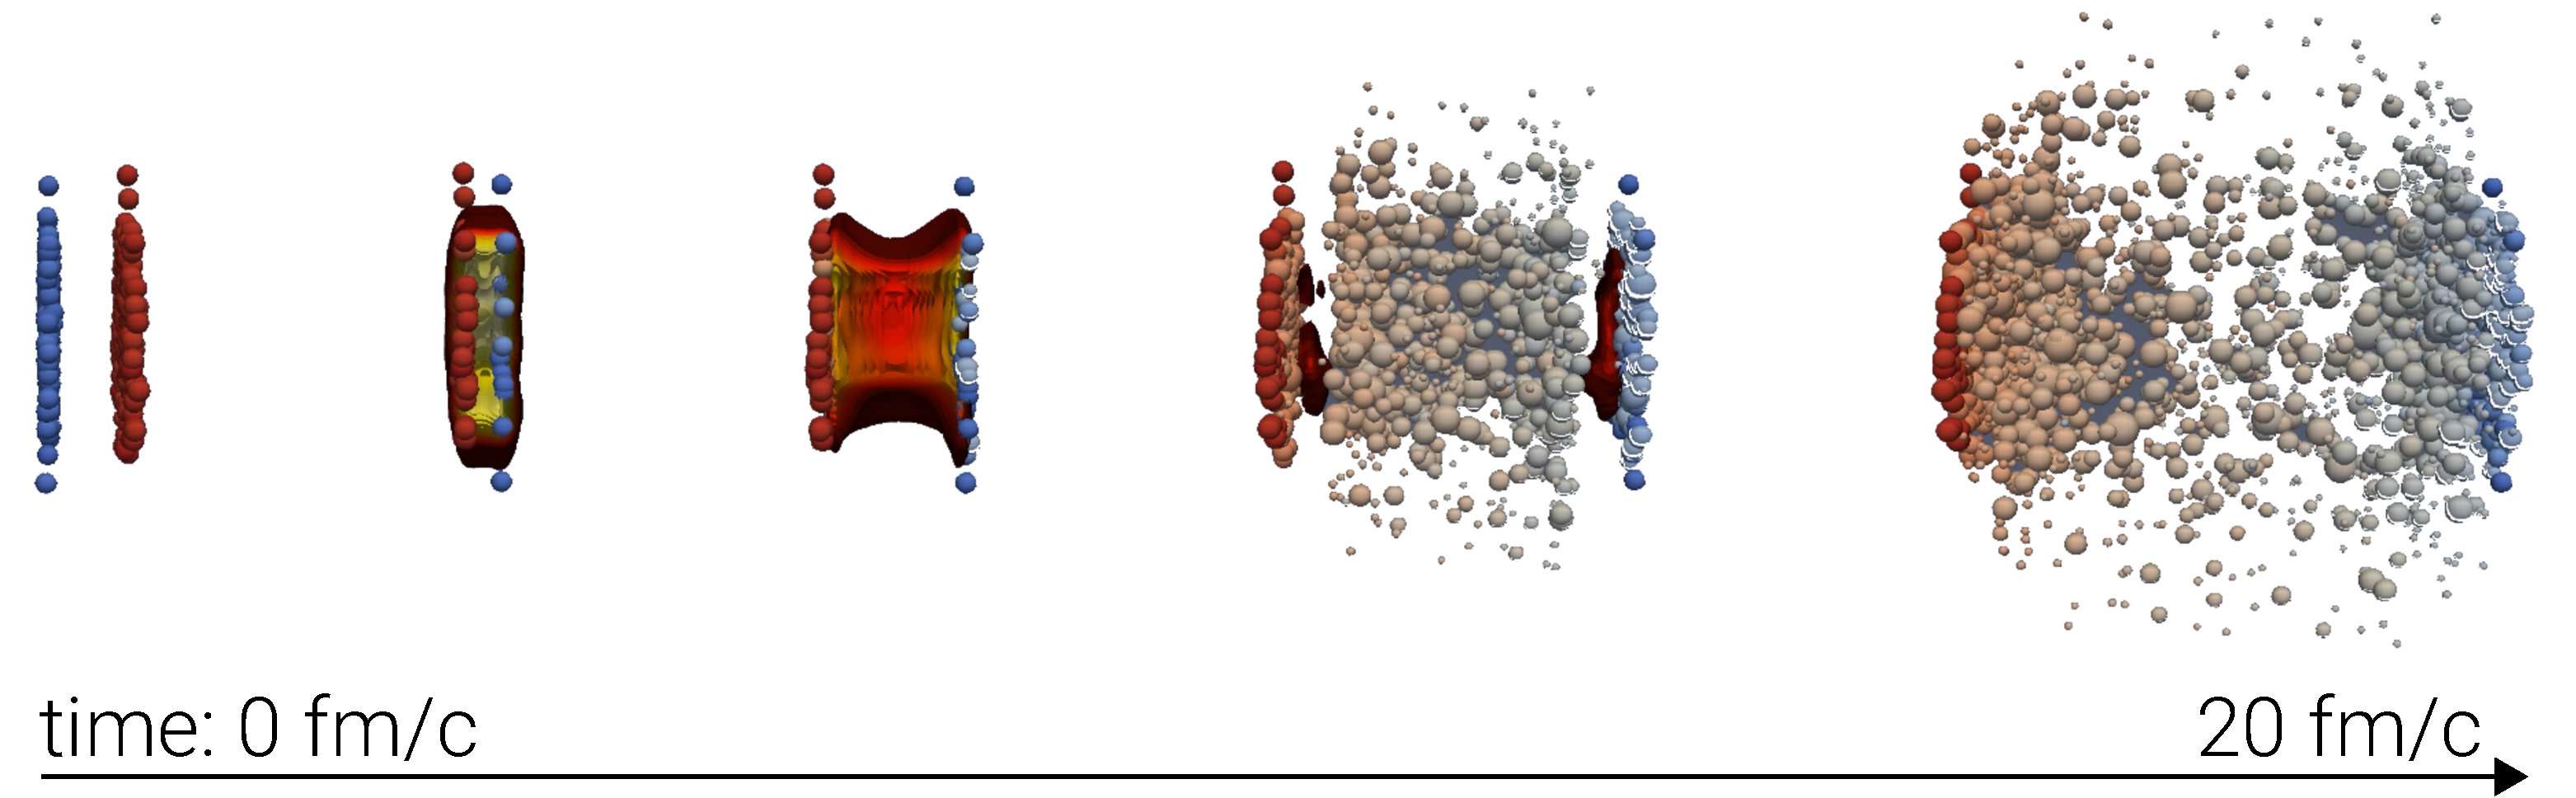
\includegraphics[width=\textwidth]{hic_picture1}\\
    \scriptsize
    Hydro framework imposes local energy and momentum conservation.\\
    Clearly breaks in dilute limit. Should apply with care.
  }

  \only<2>{
  \begin{tcolorbox}[colback=theme!10, colframe=theme!0]
    \begin{itemize}
      \small
      \item[\color{offblack} \scriptsize \faicon{exclamation-triangle}] Hydro for heavy-ion collisions not trusted on same level as e.g.\ GR for gravitational waves
      \item Hydro overwhelmingly supported by empirical evidence
      \item Posterior results \underline{always} subject to framework credibility
      \item Known-unknowns are quantifiable in the posterior, unknown-unknowns are not!
    \end{itemize}
  \end{tcolorbox}}
\end{frame}

\begin{frame}{Seminal Bayesian works in heavy-ion physics}
  \begin{columns}[T]
    \begin{column}{0.5\textwidth}
      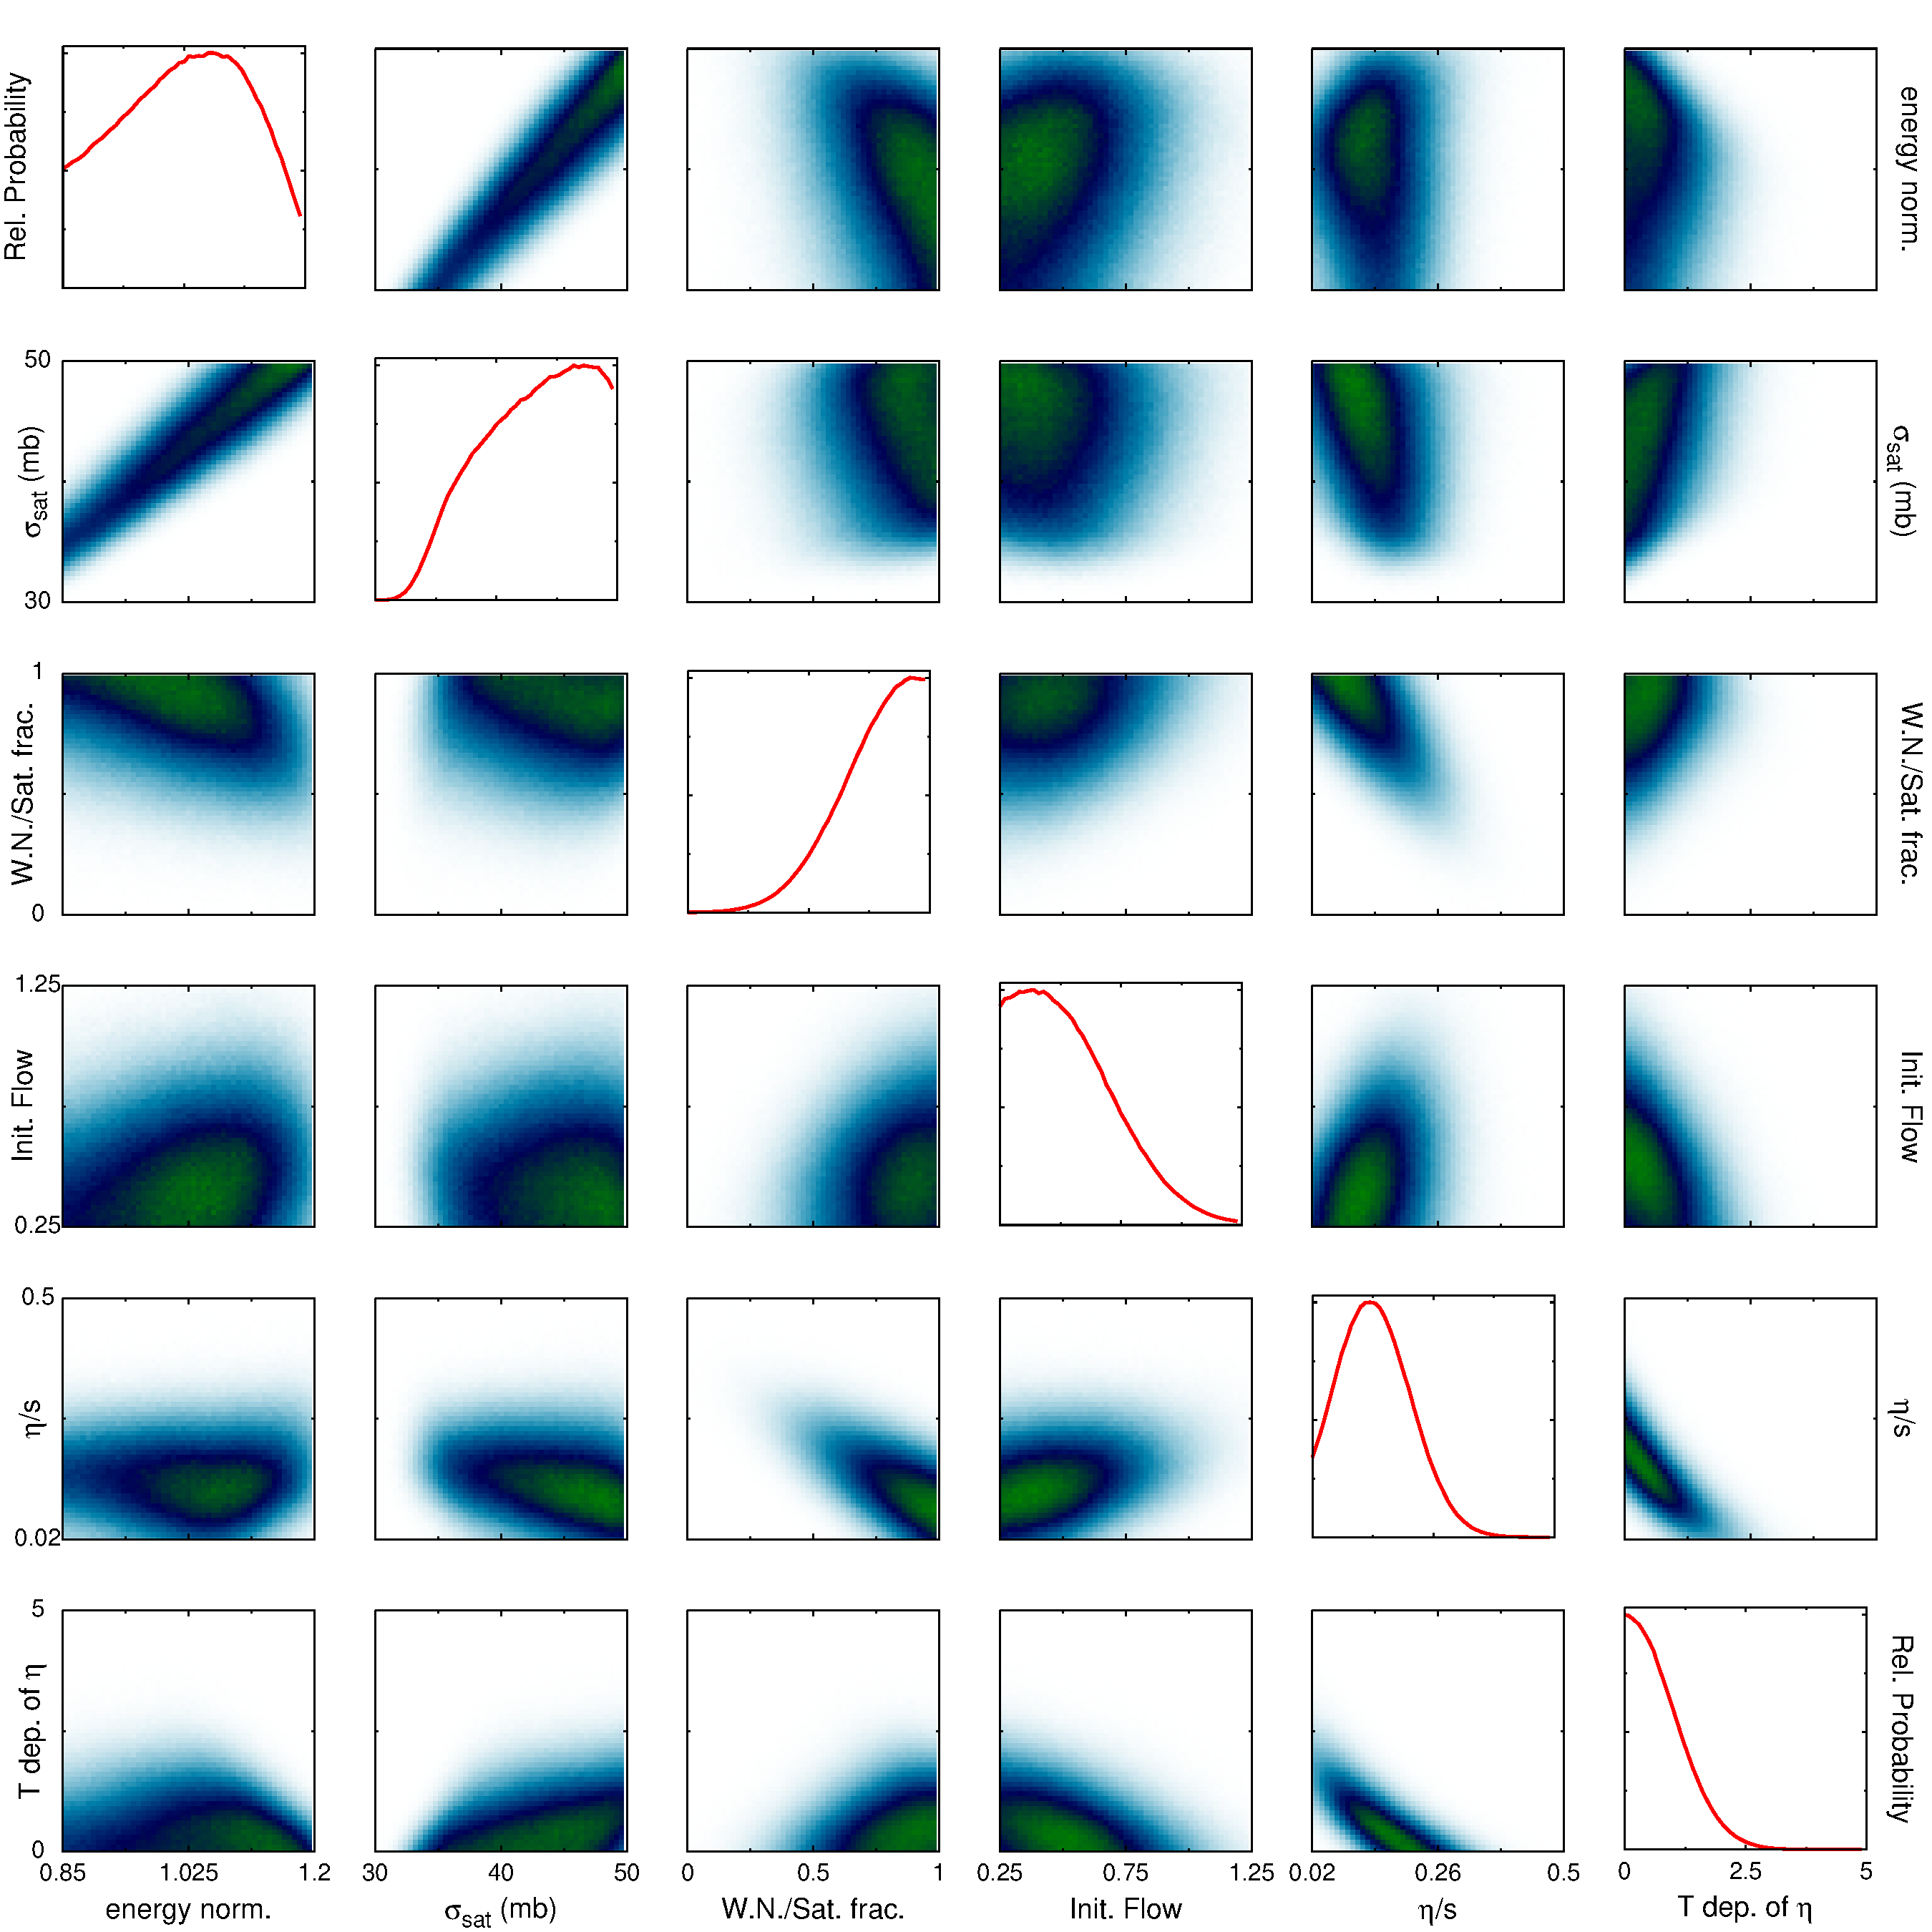
\includegraphics[width=\textwidth]{pratt_fig11}
    \end{column}
    \begin{column}{0.5\textwidth}
      \begin{itemize}
        \item Event-averaged hydro
        \item Parametric pre-flow
        \item Parametric initial state
        \item First Bayesian posterior on $(\eta/s)(T)$
        \item Omits bulk viscosity
        \item Two centrality bins
      \end{itemize}
    \end{column}
  \end{columns}
  \vspace{1cm}
  \begin{columns}[T]
    \begin{column}{0.025\textwidth}
    \end{column}
    \begin{column}{0.05\textwidth}
      \raggedleft
      
\includegraphics[width=\columnwidth]{michigan-state}\\
      
\includegraphics[width=.8\columnwidth]{duke}
    \end{column}
    \begin{column}{0.9\textwidth}
      \scriptsize \setstretch{1.2}
      \textbf{Determining Fundamental Properties of Matter Created in Ultrarelativistic Heavy-Ion Collisions}, Novak, Novak, Pratt, Vredevoogd, Coleman-Smith, Wolpert
      PRC 89 (2014) 034917
    \end{column}
    \begin{column}{0.025\textwidth}
    \end{column}
  \end{columns}
\end{frame}

\begin{frame}{Seminal Bayesian works in heavy-ion physics}
  \begin{itemize}
    \item Equation of state from lattice QCD is very close to parametric equation of state preferred by simulation
  \end{itemize}
  \begin{center}
    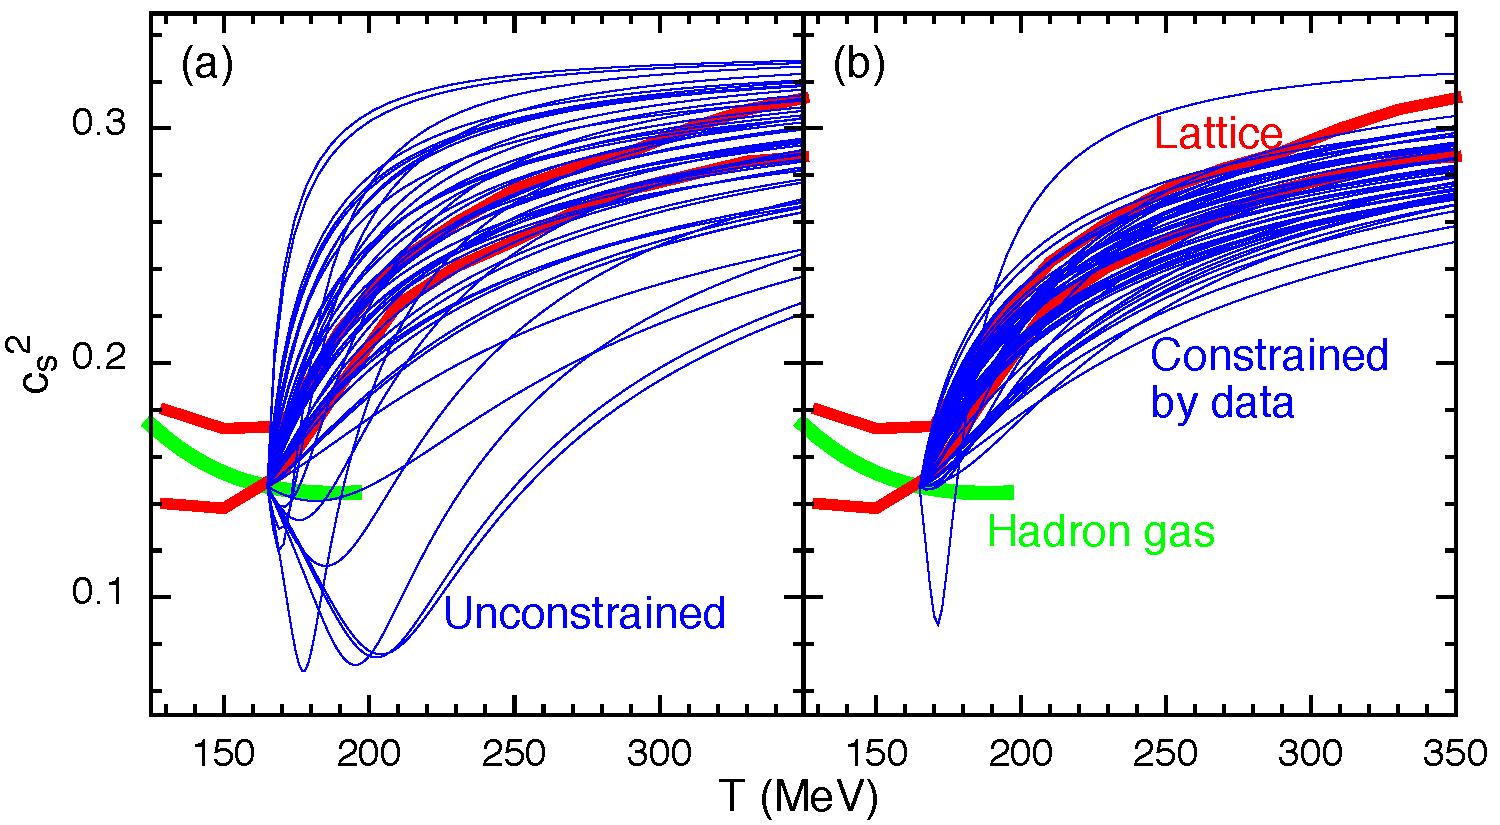
\includegraphics[width=.8\textwidth]{priorvpost50}
  \end{center}
  \begin{columns}[T]
    \begin{column}{0.025\textwidth}
    \end{column}
    \begin{column}{0.05\textwidth}
      \raggedleft
      
\includegraphics[width=\columnwidth]{michigan-state}\\[-0.5ex]
      \textbf{\small BNL}
    \end{column}
    \begin{column}{0.9\textwidth}
      \scriptsize \setstretch{1.2}
      \textbf{Constraining the Eq.\ of State of Super-Hadronic Matter from Heavy-Ion Collisions}, Pratt, Sangaline, Sorensen, Wang, PRL 114 (2015) 202301
    \end{column}
    \begin{column}{0.025\textwidth}
    \end{column}
  \end{columns}

\end{frame}

\begin{frame}{Seminal Bayesian works in heavy-ion physics}
  \begin{columns}[T]
    \begin{column}{0.55\textwidth}
      \centering
      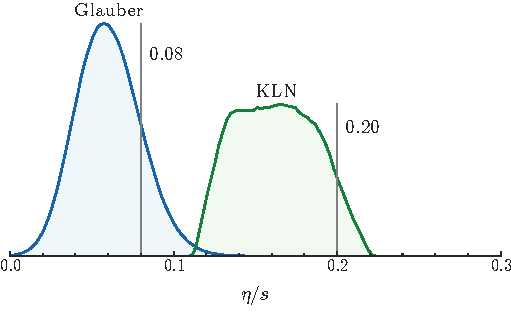
\includegraphics[width=\textwidth]{post_compare}\\
      {\scriptsize Theoretical biases affect preferred viscosity}
    \end{column}
    \begin{column}{0.45\textwidth}
      \begin{itemize}
        \item Event-by-event hydro
        \item MC-Glauber \& KLN initial conditions
        \item Centrality bins like experiment
        \item Constant $\eta/s$
        \item Omits bulk viscosity, pre-flow
      \end{itemize}
    \end{column}
  \end{columns}
  \vspace{1cm}
  \begin{columns}[T]
    \begin{column}{0.025\textwidth}
    \end{column}
    \begin{column}{0.05\textwidth}
      \raggedleft
      
\includegraphics[width=.8\columnwidth]{duke}
    \end{column}
    \begin{column}{0.9\textwidth}
      \scriptsize \setstretch{1.2}
      \textbf{Constraining the Eq.\ of State of Super-Hadronic Matter from Heavy-Ion Collisions}, Bernhard, Marcy, Coleman-Smith, Huzurbazar, Wolpert, Bass, PRC 91 (2015) 054910
    \end{column}
    \begin{column}{0.025\textwidth}
    \end{column}
  \end{columns}

\end{frame}

\begin{frame}{Towards precision extraction of QGP properties}
  \begin{columns}[T]
    \begin{column}{0.025\textwidth}
    \end{column}
    \begin{column}{0.05\textwidth}
      \raggedleft
      
\includegraphics[width=\columnwidth]{duke}\\[.5ex]
      
\includegraphics[width=.9\columnwidth]{osu}
    \end{column}
    \begin{column}{0.9\textwidth}
      \scriptsize \setstretch{1.2}
      \textbf{Applying Bayesian parameter estimation to relativistic heavy-ion collisions: simultaneous characterization of the initial state and QGP medium},\\
      Bernhard, Moreland, Bass, Liu, Heinz PRC 94 (2016) 024907
    \end{column}
    \begin{column}{0.025\textwidth}
    \end{column}
  \end{columns}
  \begin{columns}[T]
    \begin{column}{.5\textwidth}
      \begin{center}
      \begin{block}{Generational improvements}
        \begin{itemize}
          \scriptsize 
          \item New \textbf{\trento} initial condition model: absorbs initial state uncertainties into several free parameters
          \item Full event-by-event hydro with hadronic afterburner
          \item Calculate observables exactly as experiment
          \item Bulk and shear viscous corrections
          \item \emph{More} experimental observables
        \end{itemize}
      \end{block}
      \end{center}
    \end{column}
    \begin{column}{.5\textwidth}
      \begin{center} 
        {\scshape Physics insights}\\[1ex]
        $\eta/s~\text{min} = 0.07 \pm 0.05$ \\
        non-zero bulk viscosity\\[2ex]
        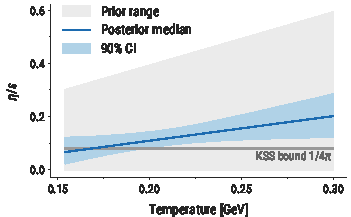
\includegraphics[width=\columnwidth]{etas_estimate}
      \end{center}
    \end{column}
  \end{columns}
\end{frame}


\begin{frame}{Towards precision extraction of QGP properties}
  \begin{columns}[T]
    \begin{column}{0.025\textwidth}
    \end{column}
    \begin{column}{0.05\textwidth}
      \raggedleft
      
\includegraphics[width=\columnwidth]{duke}\\[.5ex]
      
\includegraphics[width=.9\columnwidth]{osu}
    \end{column}
    \begin{column}{0.9\textwidth}
      \scriptsize \setstretch{1.2}
      \textbf{Applying Bayesian parameter estimation to relativistic heavy-ion collisions: simultaneous characterization of the initial state and QGP medium},\\
      Bernhard, Moreland, Bass, Liu, Heinz PRC 94 (2016) 024907
    \end{column}
    \begin{column}{0.025\textwidth}
    \end{column}
  \end{columns}

  \begin{center}
    {\small Model calculations with high-likelihood parameters from Bayesian posterior
    provide excellent description of bulk observables}\\[1ex]
    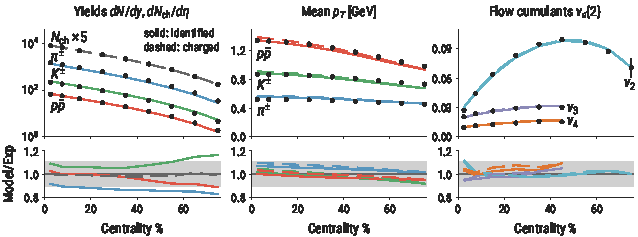
\includegraphics{mode_observables}
  \end{center}
\end{frame}


\begin{frame}{Bulk viscosity: a work in progress...}{}
  \medskip
  {\scshape Challenges}
  \begin{itemize}
    \small
    \item Different methods for bulk viscous corrections at freezeout
    \item Less obvious parametric form for $(\zeta/s)(T)$
    \item Hydro breaks (cavitates) if bulk is too large 
  \end{itemize}
  \vspace{.5cm}

  \begin{columns}[b]
    \begin{column}{.38\textwidth}
      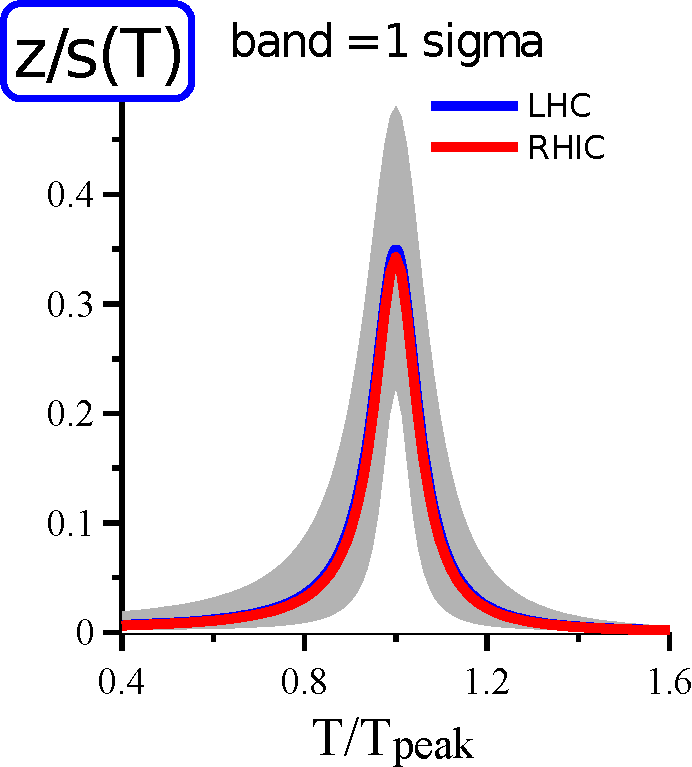
\includegraphics[width=\columnwidth]{gabriel_bulk}
    \end{column}
    \begin{column}{.62\textwidth}
      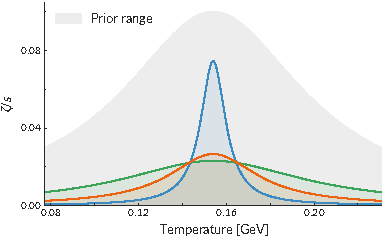
\includegraphics[width=\columnwidth]{jbernhard_qm2017}\\
    \end{column}
  \end{columns}

  \begin{columns}[b]
    \begin{column}{.38\textwidth}
      \centering \scriptsize Denicol, Paquet, Gale, Jeon, Shen
    \end{column}
    \begin{column}{.62\textwidth}
      \centering \scriptsize Bernhard, Moreland, Bass
    \end{column}
  \end{columns}
\end{frame}

\begin{frame}{Studying the QGP fireball in 3D}
  \begin{center}
    Initial energy density (2D)\\[.5ex]
    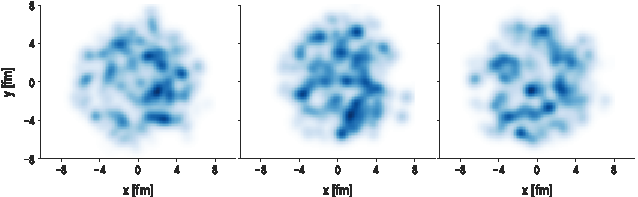
\includegraphics[width=.6\textwidth]{trento2d}\\[1ex]
    Initial energy density (3D)\\[.5ex]
    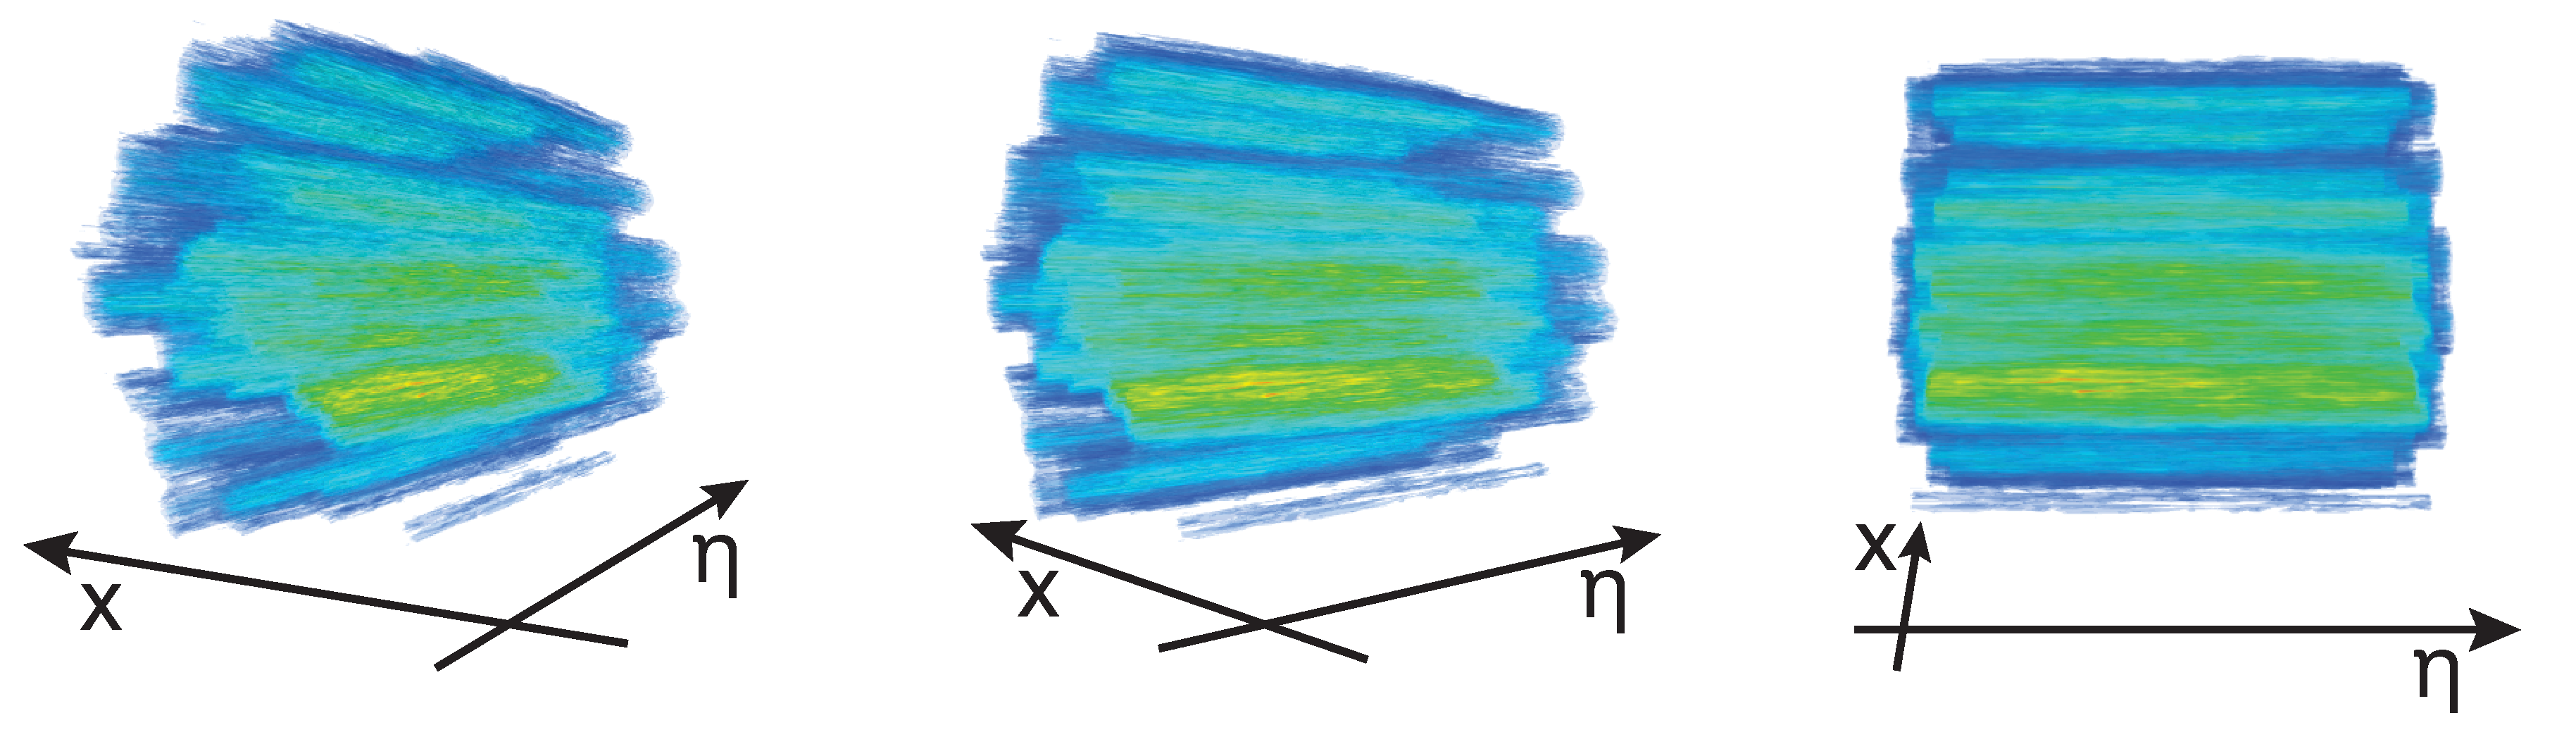
\includegraphics[width=.8\textwidth]{three_dim}\\
    {\tiny Figure credit: Schenke, Schlichting}
  \end{center}
\end{frame}


\begin{frame}{Studying the QGP fireball in 3D}
  \bigskip
  \begin{columns}[T]
    \begin{column}{0.025\textwidth}
    \end{column}
    \begin{column}{0.05\textwidth}
      \raggedleft
      
\includegraphics[width=\columnwidth]{duke}
    \end{column}
    \begin{column}{0.9\textwidth}
      \scriptsize \setstretch{1.2}
      \textbf{Constraints on rapidity-dependent initial conditions from charged particle pseudorapidity densities and two-particle correlations},\\
      Ke, Moreland, Bernhard, Bass (in prep)
    \end{column}
    \begin{column}{0.025\textwidth}
    \end{column}
  \end{columns}
  \vspace{-.5cm}
  \begin{columns}
    \begin{column}{.5\textwidth}
      \begin{block}{Optimization problem}
        \small
        Find initial energy density that evolves into final single particle distribution
      \end{block}
      \begin{itemize}
        \small
        \item Parametrize initial longitudinal energy profile with moment-generating function\\[1ex]
        \item Constrain form using charged particle rapidity distributions\\[1ex]
      \end{itemize}
    \end{column}
    \begin{column}{.5\textwidth}
      \begin{center}
        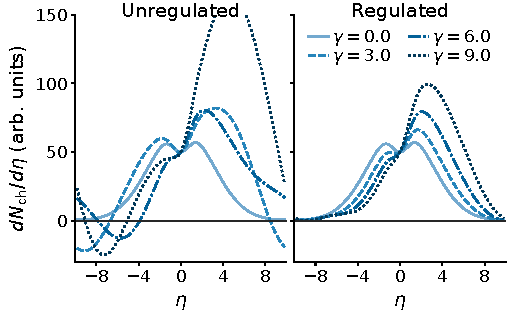
\includegraphics[width=.8\columnwidth]{regulate}\\[.5ex]
        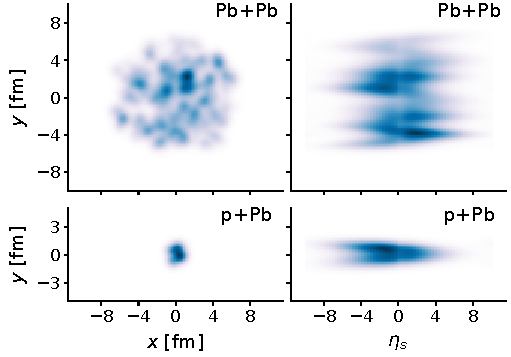
\includegraphics[width=.9\columnwidth]{trento3d_example}
      \end{center}
    \end{column}
  \end{columns}
\end{frame}

\begin{frame}{Studying the QGP fireball in 3D}
  \vspace{1cm}
  \begin{tikzpicture}[remember picture, overlay]
    \node (x1) at (2.5, -0.5) {};
    \node (x2) at (8.2, -0.5) {};
    \node at (5.5, .8) {Bayesian analysis};
    \draw[->, thick] (x2.north) to [out=150, in=30] (x1.north);
  \end{tikzpicture}
  \begin{columns}
    \begin{column}{.4\textwidth}
      \begin{center}
        Initial entropy profile\\
        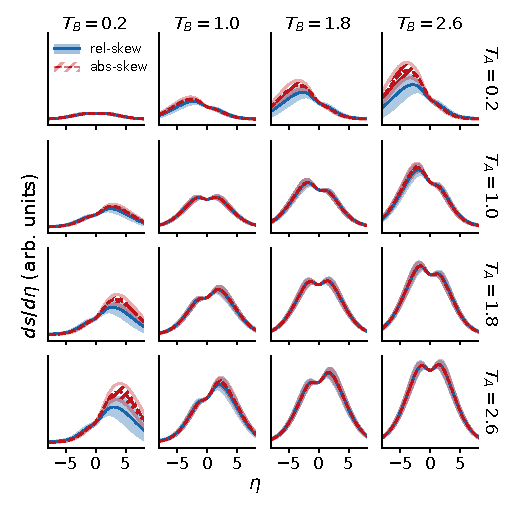
\includegraphics[width=\textwidth]{post_dsdy}
      \end{center}
    \end{column}
    \begin{column}{.6\textwidth}
      \begin{center}
        Final particle distribution\\
        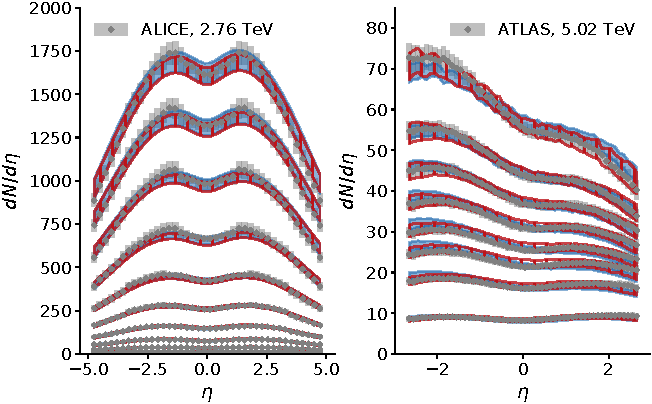
\includegraphics[width=\textwidth]{post_obs}
      \end{center}
    \end{column}
  \end{columns}
  \begin{itemize}
    \item Trust in hydro and Bayesian statistical machinery let's us deconvolve complex system evolution
  \end{itemize}
\end{frame}

\begin{frame}{QGP hard probes: open heavy-flavour}
  \begin{tikzpicture}[remember picture, overlay]
    \node[rotate=45] at (0.3, -.5) {\color{pyred} \bf Analogue};
  \end{tikzpicture}
  \begin{center}
    \begin{tabular}{ll}
      Theory framework & Free parameter(s)\\
      \noalign{\smallskip}\hline\noalign{\smallskip}
      \small Hydrodynamics & \small QGP viscosity: $\eta/s$, $\zeta/s$\\[.5ex]
      \small Langevin transport & \small charm diffusion coefficient: $D_{s,p}$
  \end{tabular}
  \end{center}
  \vspace{.5cm}
  \begin{columns}[T]
    \begin{column}{.55\textwidth}
      \centering \small QGP shear viscosity\\[.5ex]
      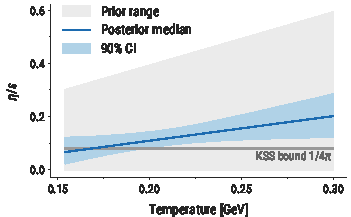
\includegraphics[width=\textwidth]{etas_estimate}
    \end{column}
    \begin{column}{.45\textwidth}
      \centering \small Charm diffusion coefficient\\[.5ex]
      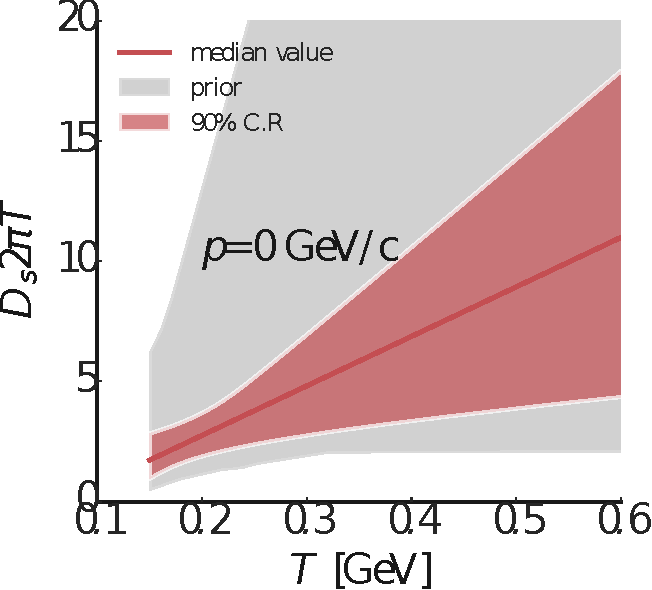
\includegraphics[width=.9\textwidth]{Plot_D2piT_posterior_T}
    \end{column}
  \end{columns}
  \begin{flushleft}
    \scriptsize
    \textbf{A data driven analysis for the temperature and momentum dependence of the heavy quark diffusion coefficient in relativistic heavy-ion collisions}\\
    Xu, Bernhard, Bass, Nahrgang, Cao (in preparation)
  \end{flushleft}
\end{frame}

\appendix

\begin{frame}[plain, noframenumbering]
  \begin{center}
    \scshape Backup slides
  \end{center}
\end{frame}


\begin{frame}{Seminal Bayesian works in heavy-ion physics}
  \vspace{-.5cm}
  \begin{center}
    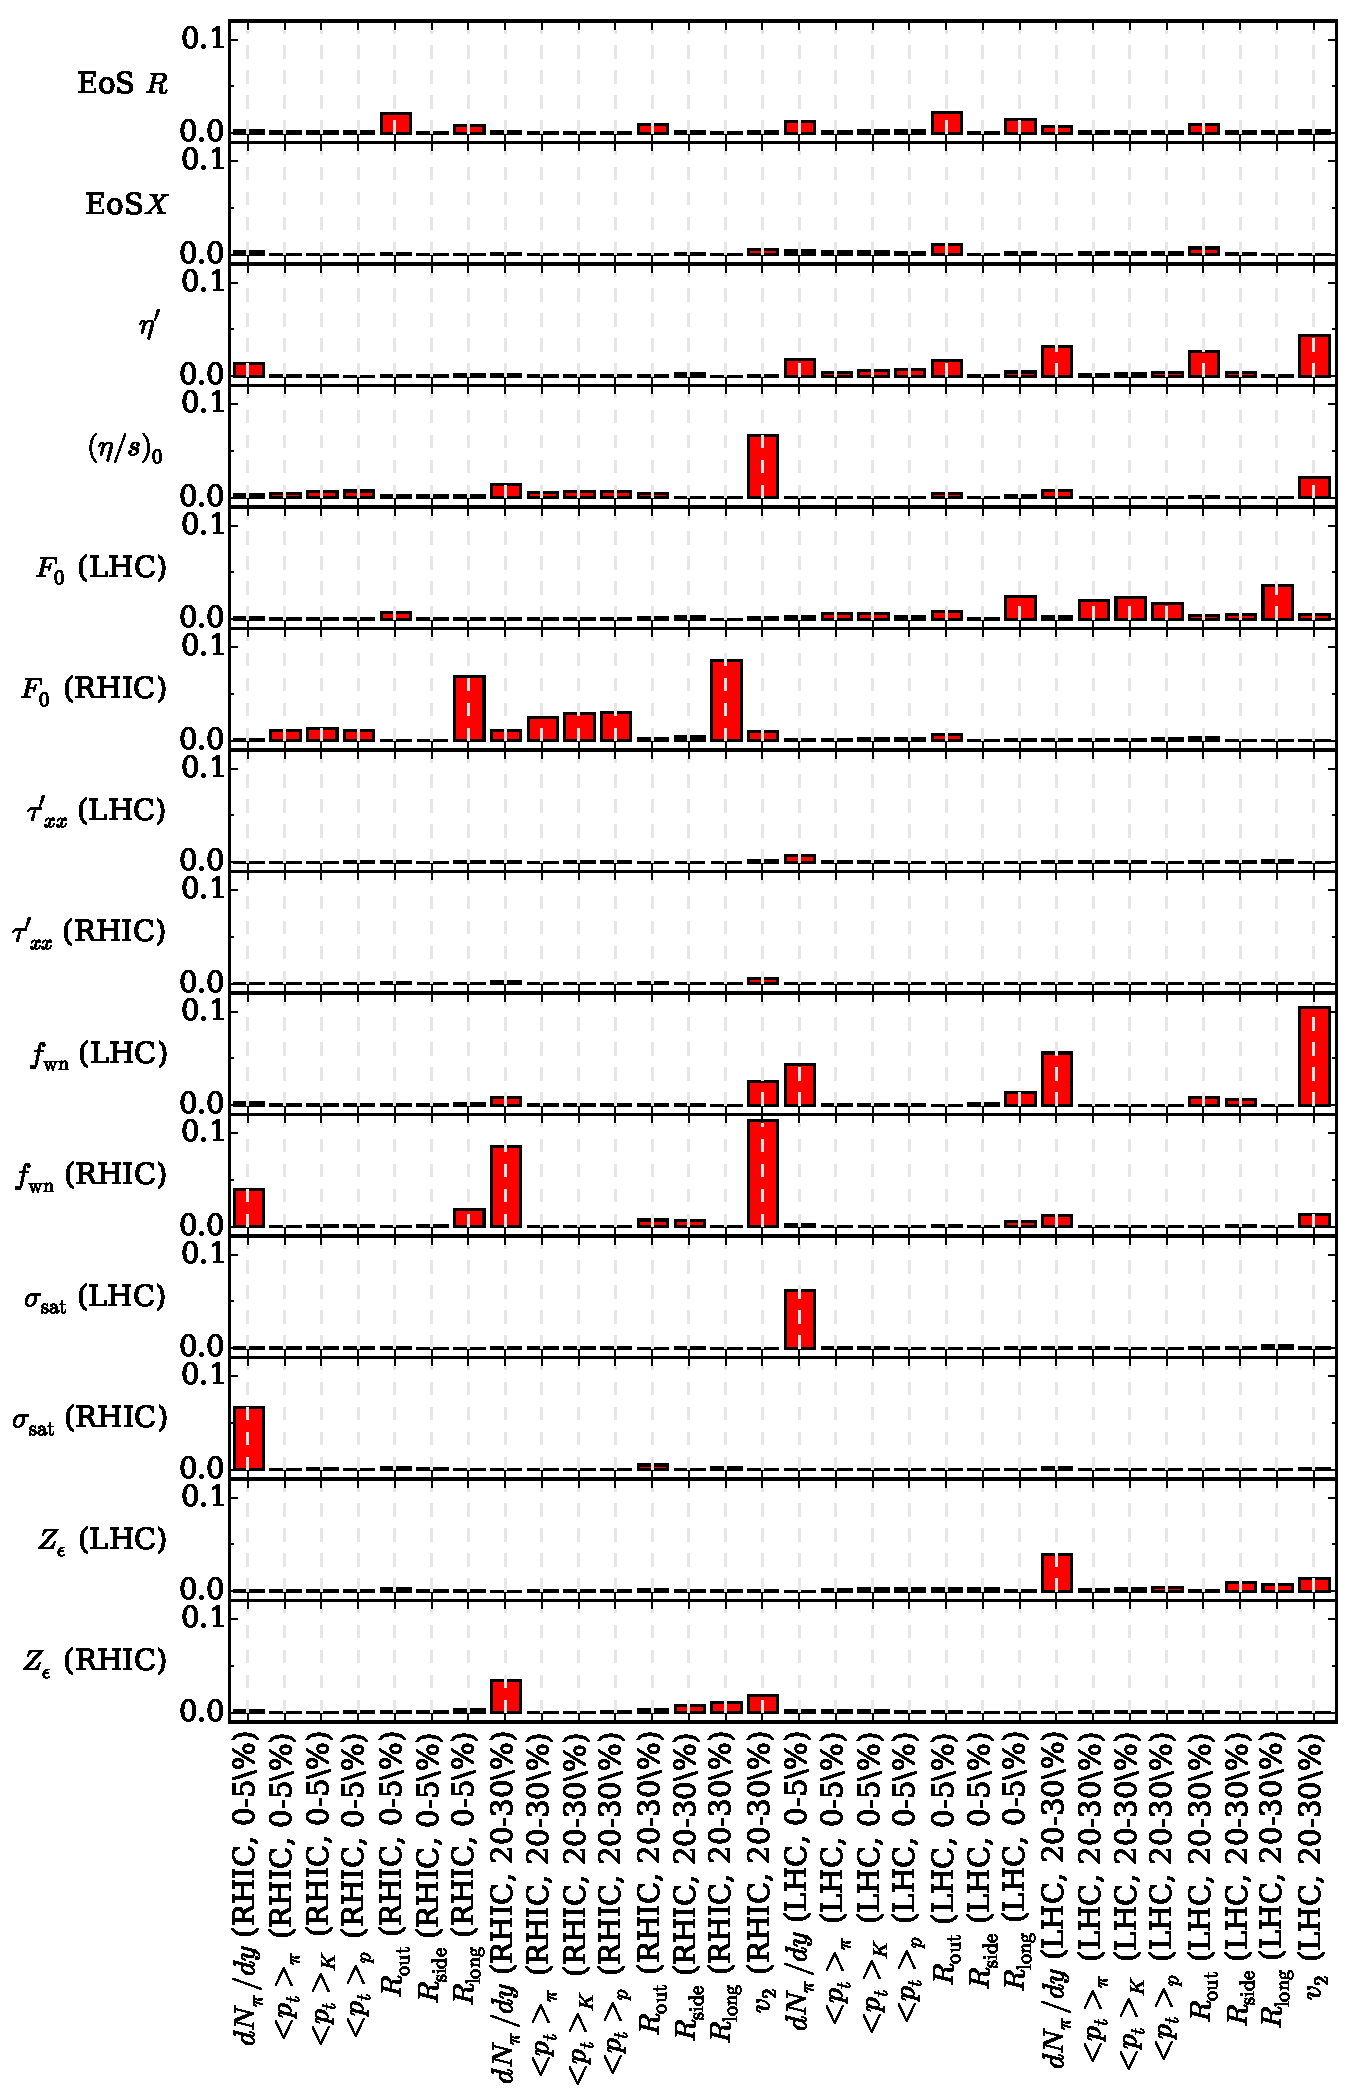
\includegraphics[width=0.5\textwidth, rotate=-90]{sensitivity}\\[.5ex]
    \scriptsize Sensitivity of experimental observables to model parameters
  \end{center}
  \begin{columns}[T]
    \begin{column}{0.025\textwidth}
    \end{column}
    \begin{column}{0.05\textwidth}
      \raggedleft
      
\includegraphics[width=\columnwidth]{michigan-state}
    \end{column}
    \begin{column}{0.9\textwidth}
      \scriptsize \setstretch{1.2}
      \textbf{Towards a Deeper Understanding of How Experiments Constrain the Underlying Physics of Heavy-Ion Collisions}, Sangaline, Pratt, PRC 93 (2016) 024908
    \end{column}
    \begin{column}{0.025\textwidth}
    \end{column}
  \end{columns}

\end{frame}

\end{document}
